% HMC Math dept HW template example
% v0.04 by Eric J. Malm, 10 Mar 2005
\documentclass[10pt,a4paper,boxed]{hmcpset}

% set 1-inch margins in the document
% \usepackage[margin=1in]{geometry}
\usepackage{enumerate}
\usepackage{todonotes}
%\usepackage{tikz}
%\usetikzlibrary{positioning}
\usepackage{subfig} % subfigures in figures.	
\usepackage{pgfplots}
\usepackage{amsmath}
\usepackage{amsfonts}
\usepackage{amssymb}

%% work around for subfig and asy environment
\makeatletter
\newsavebox{\sfe@box}
\newenvironment{subfloatenv}[2]{%
\def\sfe@caption{#1}%
\def\sfe@label{#2}%
\setbox\sfe@box\hbox\bgroup\color@setgroup}%
{\color@endgroup\egroup\subfloat[\sfe@caption]%
{\usebox{\sfe@box}\label{\sfe@label}}}
\makeatother

% include this if you want to import graphics files with /includegraphics
\usepackage{graphicx}

\renewcommand*{\familydefault}{\sfdefault}
\newcommand{\vect}[1]{\mathbf{#1}}


%\tikzset{node distance=2cm, inner/.style={draw,circle}, leaf/.style={draw,rectangle}}

\usepackage{hyperref}

% info for header block in upper right hand corner
\name{Lukas Gesing, Patrick Kaster}
\class{MA-INF 4201 - Artificial Life}
\assignment{Exercise Sheet 7}
% \duedate{09/03/2004}

\begin{document}


\begin{problem}[Assignment 44]
\end{problem}
\begin{solution}
Assuming that the rules for the $2$-point-cross-over recombination-operator are analogous to the $1$-point-cross-over recombination-operator there can only be two cases:
The genome is split at two points. Either:
\begin{enumerate}
	\item The part up to point $1$ is taken from parent $A$, the part between point $1$ and point $2$ is taken from parent $B$ and the final part from point $2$ to the end is again taken from parent $A$.
	\item or the part up to point $1$ is taken from parent $B$, the part between point $1$ and point $2$ is taken from parent $A$ and the final part from point $2$ to the end is again taken from parent $B$.
\end{enumerate}
So, regardless of the genome sequence length $L$, there can only be two different offsprings. Thus, the diversity of the population has to be provided by the size of the population or a mutation operator.

\end{solution}

\begin{problem}[Assignment 45]
\end{problem}
\begin{solution}
A binary genome of length $L$ can be represented by a hypercube of dimension $L$ of unit edge length. Every bit of the genome corresponds to an axis of the hypercube. Since the hypercube has unit edge length and the genome is binary, a genome corresponds to a specific corner of the hypercube. This is depicted for the three-bit-genomes $(0,0,1), (1,1,0), (1,0,1)$ in figure (\ref{fig:hypercube}).

\begin{figure}[h!]
	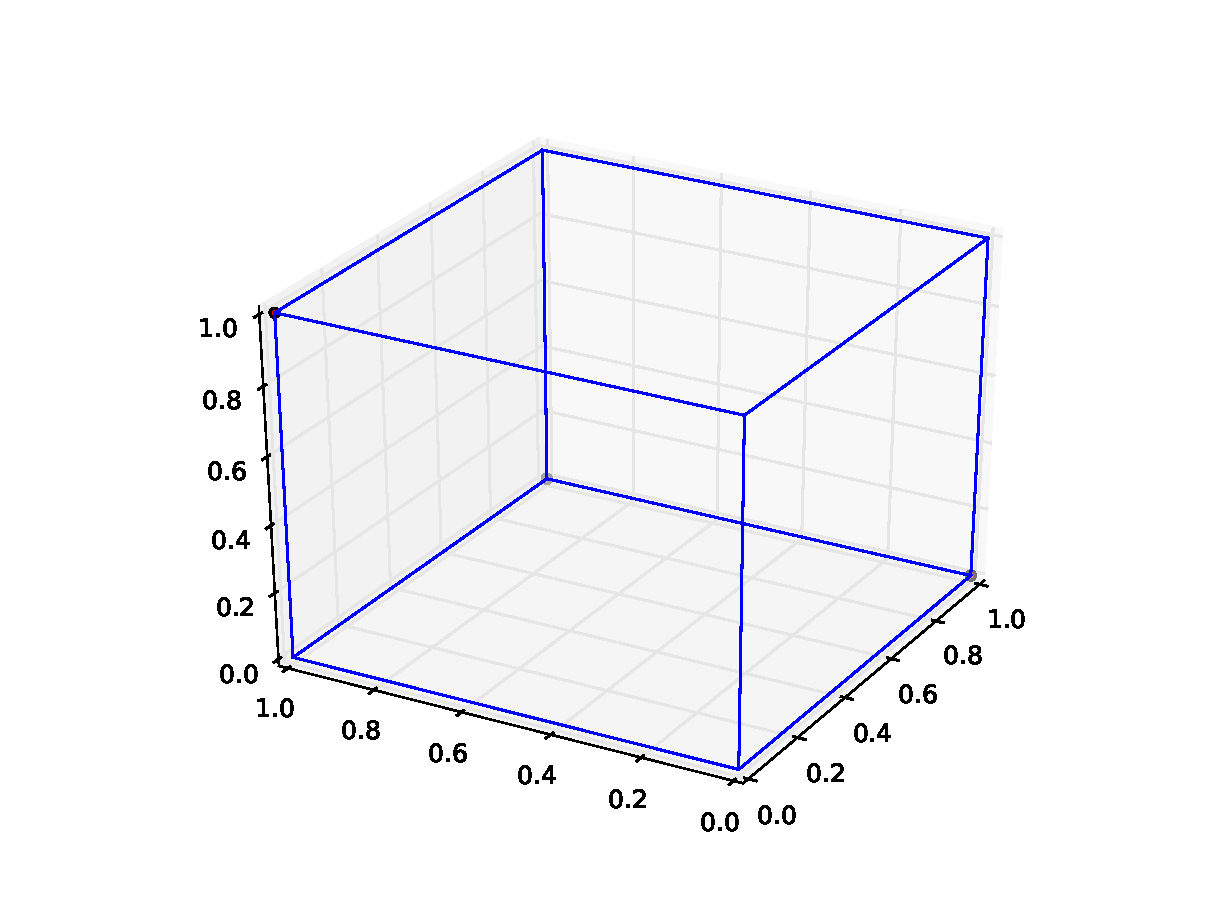
\includegraphics[width=\textwidth]{img/cube}
\caption{representation of three-bit-genomes by an three dimensional hypercube}
\label{fig:hypercube}
\end{figure}
\end{solution}

\begin{problem}[Assignment 46]
\end{problem}
\begin{solution}
Generating all possible sequences of L is equivalent to finding all permutations of L. Since every permutation can be expressed as a product of transpositions (the swapping of two elements), the algorithm can generate all sequences.
\end{solution}

\begin{problem}[Assignment 47]
\end{problem}
\begin{solution}
Done, needs further explanation $1-(N \cdot (1-p)^L)$
\end{solution}

\begin{problem}[Assignment 48]
\end{problem}
\begin{solution}
\emph{External selection} selects the individuals to "survive", while the rest of the population is discarded. \emph{Parent selection} selects those "survivors" which will generate new offspring to replenish the population.
\end{solution}

\begin{problem}[Assignment 49]
\end{problem}
\begin{solution}
\end{solution}


\end{document}
